% !TEX program = xelatex
% Build: latexmk -xelatex main.tex
\documentclass[aspectratio=169,11pt]{beamer}

\usetheme[progressbar=frametitle,numbering=fraction,block=fill]{metropolis}

\usepackage{amsmath,amssymb,bm}
\usepackage{booktabs,array,tabularx}
\usepackage{tikz}
\usetikzlibrary{arrows.meta,positioning,calc,fit}
\usepackage{tcolorbox}
\tcbuselibrary{skins}

% ---------- colors ----------
\definecolor{ink}{HTML}{1F2A37}
\definecolor{accent}{HTML}{C2410C}
\definecolor{cBlue}{HTML}{2563EB}
\definecolor{cGreen}{HTML}{15803D}
\definecolor{cPurple}{HTML}{7C3AED}
\definecolor{cRed}{HTML}{B91C1C}
\definecolor{cGray}{HTML}{6B7280}
\definecolor{cTeal}{HTML}{0F766E}
\definecolor{soft}{HTML}{F3F4F6}

\setbeamercolor{frametitle}{bg=ink,fg=white}
\setbeamercolor{progress bar}{fg=accent,bg=ink!30}
\setbeamercolor{title separator}{fg=accent}
\setbeamercolor{alerted text}{fg=accent}
\setbeamercolor{normal text}{fg=ink,bg=white}
\setbeamercolor{block title}{bg=ink!12,fg=ink}
\setbeamercolor{block body}{bg=soft}
\setbeamercolor{block title alerted}{bg=accent!18,fg=accent!80!black}
\setbeamercolor{block body alerted}{bg=accent!5}
\setbeamercolor{block title example}{bg=cGreen!15,fg=cGreen!80!black}
\setbeamercolor{block body example}{bg=cGreen!4}
\setbeamertemplate{itemize item}{\color{accent}$\blacktriangleright$}
\setbeamertemplate{itemize subitem}{\color{cGray}--}
\metroset{sectionpage=progressbar}

% ---------- notation ----------
\newcommand{\E}{\mathbb{E}}
\newcommand{\pit}{\pi_\theta}
\newcommand{\pitea}{\pi_{\bar\theta}}
\newcommand{\piold}{\pi_{\mathrm{old}}}
\newcommand{\sg}{\operatorname{sg}}
\newcommand{\KL}{D_{\mathrm{KL}}}
\newcommand{\Ind}{\mathbb{I}}
\newcommand{\abs}[1]{\lvert #1\rvert}
\newcommand{\norm}[1]{\lVert #1\rVert}
\newcommand{\acc}{\operatorname{acc}}
\newcommand{\ans}{\operatorname{ans}}
\newcommand{\pct}{\operatorname{p}_{99}}
\newcommand{\AUROC}{\operatorname{AUROC}}
\newcommand{\dm}{d_{\mathrm{model}}}
\newcommand{\hl}[1]{{\color{accent}#1}}
\newcommand{\gnote}[1]{{\scriptsize\color{cGray}#1}}

% ---------- cost tags ----------
\newcommand{\ctag}[2]{\tikz[baseline=(T.base)]\node[fill=#1!14,text=#1!75!black,
  rounded corners=1.5pt,inner xsep=2.5pt,inner ysep=1.2pt,font=\scriptsize\bfseries](T){#2};}
\newcommand{\cFree}{\ctag{cGreen}{free}}
\newcommand{\cFwd}{\ctag{cBlue}{+fwd}}
\newcommand{\cLog}{\ctag{cPurple}{logits}}
\newcommand{\cGrad}{\ctag{accent}{grad}}
\newcommand{\cEval}{\ctag{cGray}{eval}}
\newcommand{\cOff}{\ctag{ink}{offline}}
\newcommand{\cRun}{\ctag{cRed}{+run}}
\newcommand{\cBr}{\ctag{cTeal}{branch}}

% ---------- tables ----------
\newcolumntype{Y}{>{\raggedright\arraybackslash}X}
\newenvironment{stattable}[1][2.1cm]{%
  \scriptsize\setlength{\tabcolsep}{4pt}\renewcommand{\arraystretch}{1.22}%
  \tabularx{\linewidth}{@{}>{\raggedright\arraybackslash\bfseries}p{#1} Y
    >{\centering\arraybackslash}p{1.05cm} >{\raggedright\arraybackslash}p{2.9cm}@{}}
  \toprule
  \normalfont\bfseries Statistic & \bfseries Definition / procedure & \bfseries Cost & \bfseries What it tells you\\
  \midrule}
 {\bottomrule\endtabularx}

\newenvironment{symtable}{%
  \footnotesize\setlength{\tabcolsep}{4pt}\renewcommand{\arraystretch}{1.12}%
  \tabularx{\linewidth}{@{}>{\raggedright\arraybackslash}p{0.40\linewidth} Y@{}}
  \toprule \textbf{Symbol} & \textbf{Meaning}\\ \midrule}
 {\bottomrule\endtabularx}

% equation box
\newtcolorbox{eqbox}[1][]{enhanced,colback=soft,colframe=ink!40,boxrule=0.5pt,
  arc=2pt,left=4pt,right=4pt,top=2pt,bottom=2pt,#1}

\title{Profiling On-Policy Self-Distillation}
\subtitle{General statistics for OPD / OPSD experiments, and statistics for the PMI / prefix-compatibility hypothesis}
\author{}
\date{}

\begin{document}

\maketitle

% =====================================================================
\begin{frame}{Outline}
\begin{columns}[T]
\column{0.46\textwidth}
\textbf{Part I: general statistics}\\[2pt]
\small
\begin{enumerate}
  \setlength\itemsep{0pt}
  \item[0.] Setup, notation, cost tags
  \item[A.] Sanity checks
  \item[B.] Where the signal lands
  \item[C.] Estimator quality
  \item[D.] Gradients and optimizer
  \item[E.] Calibration and confidence
  \item[F.] Representations and mechanisms
  \item[G.] Generalization, forgetting, robustness
  \item[H.] Experimental rigor
  \item[] Putting it together
\end{enumerate}
\column{0.52\textwidth}
\textbf{Part II: idea 003 (PMI, compatibility)}\\[2pt]
\small
\begin{enumerate}
  \setlength\itemsep{0pt}
  \item[II.0] Notation and hypotheses
  \item[II.1] Training health and task metrics
  \item[II.2] The per-token signal
  \item[II.3] Teacher--student distribution gap
  \item[II.4] PMI decomposition, prefix compatibility
  \item[II.5] Prefix reliability: branch continuations
  \item[II.6] Reasoning behavior and diversity
  \item[II.7] Parameter dynamics and cost
  \item[II.8] Slicing, schedule, staging
\end{enumerate}
\end{columns}
\gnote{Every symbol is defined before it is used; the appendix lists acronyms, symbols and references.}
\end{frame}

% =====================================================================
\section{Setup and Notation}

\begin{frame}{Setup: On-Policy Self-Distillation (OPSD)}
\begin{columns}[c]
\column{0.45\textwidth}
\centering
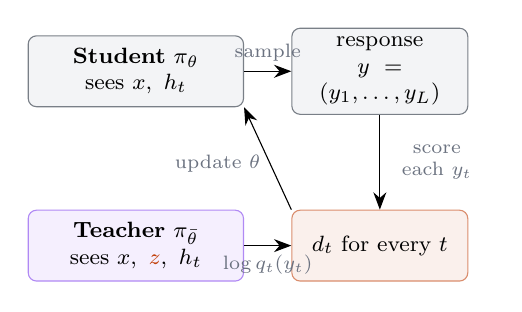
\begin{tikzpicture}[
  box/.style={draw=ink!60,rounded corners=3pt,fill=soft,align=center,
    font=\footnotesize,minimum height=0.9cm,text width=2.5cm},
  lab/.style={font=\scriptsize,color=cGray,align=center},
  >={Stealth[length=2.2mm]}]
  \node[box] (stu) {\textbf{Student} $\pit$\\ sees $x,\ h_t$};
  \node[box,below=1.3cm of stu,fill=cPurple!8,draw=cPurple!60] (tea)
    {\textbf{Teacher} $\pitea$\\ sees $x,\ \hl{z},\ h_t$};
  \node[box,right=0.6cm of stu,text width=2.0cm] (resp) {response\\ $y=(y_1,\dots,y_L)$};
  \node[box,right=0.6cm of tea,text width=2.0cm,fill=accent!8,draw=accent!60] (sig)
    {$d_t$ for every $t$};
  \draw[->] (stu) -- node[lab,above]{sample} (resp);
  \draw[->] (resp) -- node[lab,right,text width=1.2cm]{score each $y_t$} (sig);
  \draw[->] (tea) -- node[lab,below]{$\log q_t(y_t)$} (sig);
  \draw[->] (sig.north west) -- node[lab,left,pos=0.45]{update $\theta$} (stu.south east);
\end{tikzpicture}

\column{0.53\textwidth}
\footnotesize
\begin{itemize}
  \setlength\itemsep{2pt}
  \item $x$: prompt. $z$: privileged information (e.g.\ a reference solution), shown only to the teacher.
  \item The student $\pit$ (parameters $\theta$) samples a response $y=(y_1,\dots,y_L)$; $h_t=(y_1,\dots,y_{t-1})$ is the prefix before position $t$.
  \item Student: $p_t=\pit(\cdot\mid x,h_t)$.\\
    Teacher: the same network with parameters $\bar\theta$ and extra context $z$: $q_t=\pitea(\cdot\mid x,z,h_t)$.
  \item Per-token signal $d_t=\log q_t(y_t)-\log p_t(y_t)$: positive where the teacher prefers $y_t$ more than the student does.
\end{itemize}
\end{columns}
\vspace{4pt}
\gnote{Plain OPD uses the same formulas with an external teacher model in place of $\pitea(\cdot\mid x,z,h_t)$. Precise notation follows on the next five slides.}
\end{frame}

% ---------------------------------------------------------------------
\begin{frame}{Notation (1/5): prompts, responses, signals}
\begin{symtable}
$x$ & prompt (problem statement)\\
$z$ & privileged information shown only to the teacher, e.g.\ a reference solution or the final answer\\
$\mathcal V$;\ \ $a\in\mathcal V$ & vocabulary; a token\\
$G$ & number of responses sampled per prompt (group size)\\
$y^{(i)}=(y^{(i)}_1,\dots,y^{(i)}_{L_i})$,\ \ $i=1,\dots,G$ & the $i$-th response to $x$; $L_i$ is its length in tokens\\
$h^{(i)}_t=(y^{(i)}_1,\dots,y^{(i)}_{t-1})$ & prefix of response $i$ before position $t$\\
$p_{i,t}=\pit(\cdot\mid x,h^{(i)}_t)$,\ \ $q_{i,t}=\pitea(\cdot\mid x,z,h^{(i)}_t)$ & student and teacher next-token distributions\\
$d_{i,t}=\log q_{i,t}(y^{(i)}_t)-\log p_{i,t}(y^{(i)}_t)$ & per-token training signal\\
$y,\ L,\ h_t,\ p_t,\ q_t,\ d_t$ & the same objects with $i$ dropped, when only one response is involved\\
\end{symtable}
\end{frame}

% ---------------------------------------------------------------------
\begin{frame}{Notation (2/5): parameters and policies}
\begin{symtable}
$\theta$ & current student parameters\\
$\theta_k$;\ \ $\theta_0$ & parameters after $k$ optimizer steps; initial parameters\\
$\Delta\theta_k=\theta_k-\theta_{k-1}$ & the $k$-th parameter update\\
$\bar\theta$ & teacher parameters: equal to $\theta$, an exponential moving average of $\theta$, or frozen\\
$\piold$ & the policy that generated the current batch; its log-probabilities are recomputed by the training engine\\
$T$ & sampling temperature\\
$u_t\in\mathbb R^{\abs{\mathcal V}}$ & student logits at position $t$, already divided by $T$, so $p_t=\operatorname{softmax}(u_t)$, i.e.\ $p_t(a)=\exp(u_t(a))/\sum_{a'}\exp(u_t(a'))$\\
$e_a\in\mathbb R^{\abs{\mathcal V}}$ & one-hot vector of token $a$\\
\end{symtable}
\end{frame}

% ---------------------------------------------------------------------
\begin{frame}{Notation (3/5): calculus and probability}
\begin{symtable}
$\log$, $\exp$ & natural logarithm and exponential\\
$\mathbb R$ & real numbers\\
$\E$, $\Pr$ & expectation, probability\\
$\nabla_\theta$, $\nabla^2_\theta$ & gradient and Hessian with respect to $\theta$\\
$\sg(\cdot)$ & stop-gradient: the value passes through, the gradient does not\\
$\KL(p\Vert q)=\sum_{a}p(a)\log\frac{p(a)}{q(a)}$ & Kullback--Leibler divergence\\
$\Ind[\cdot]$;\ \ $\operatorname{sign}(\xi)\in\{-1,0,1\}$ & 1 if the condition holds, else 0; sign of a number $\xi$\\
$\cos(\mathbf v,\mathbf w)=\mathbf v^\top\mathbf w/(\norm{\mathbf v}\,\norm{\mathbf w})$ & cosine similarity of two vectors\\
\end{symtable}
\end{frame}

% ---------------------------------------------------------------------
\begin{frame}{Notation (4/5): norms and statistics}
\begin{symtable}
$\norm{\cdot}$,\ \ $\norm{\cdot}_F$,\ \ $\norm{\cdot}_\infty$;\ \ $\operatorname{tr}$ & Euclidean norm, Frobenius norm, largest absolute entry; matrix trace\\
$\abs{\cdot}$ & absolute value of a number; size of a set; length in tokens of a sequence\\
$\operatorname{mean}$, $\operatorname{std}$, $\pct$ & mean, standard deviation, 99th percentile of a list\\
$\AUROC(s\to c)$ & for scores $s_j$ and binary labels $c_j$: $\Pr(s_j>s_{j'}\mid c_j=1,\,c_{j'}=0)$, ties count $\tfrac12$\\
$\rho_{\mathrm S}$ & Spearman correlation: Pearson correlation of the ranks\\
\end{symtable}
\end{frame}

% ---------------------------------------------------------------------
\begin{frame}{Notation (5/5): evaluation and network internals}
\begin{symtable}
$c_i\in\{0,1\}$;\ \ $R_i$ & verifier verdict for $y^{(i)}$ (1 = correct); its scalar reward, e.g.\ $R_i=c_i$\\
$\ans(y^{(i)})$;\ \ $\mathcal S_i\subseteq\{1,\dots,L_i\}$ & extracted final answer; positions of the final-answer tokens\\
$\mathcal P$;\ \ $N$ & probe set: fixed prompts with fixed sampling seeds; it is re-run every $N$ training steps\\
$\mathcal D_{\mathrm{train}}$,\ \ $\mathcal D_{\mathrm{held}}$ & training prompts; held-out prompts from the same distribution\\
$\acc(\mathcal D)$ & pass@1 on a prompt set $\mathcal D$: mean of $c_i$ over prompts and samples (``avg@16'' when 16 samples per prompt)\\
$\ell=1,\dots,N_L$;\ \ $\dm$ & layer index and number of layers; hidden size\\
$\phi^{(\ell)}_t\in\mathbb R^{\dm}$ & hidden state at position $t$ after layer $\ell$\\
$\Phi_\ell$ & matrix whose rows are $\phi^{(\ell)}_t$ for a fixed list of probe tokens\\
\end{symtable}
\end{frame}

% ---------------------------------------------------------------------
\begin{frame}{The training loss and what it estimates}
\begin{columns}[T]
\column{0.38\textwidth}
\small
Per-token loss, in policy-gradient form:
\begin{eqbox}
\[
\mathcal L_t=-\sg(d_t)\,\log p_t(y_t)
\]
\end{eqbox}
Its expected gradient is the reverse-KL gradient:
\begin{eqbox}
\[
\E_{y_t\sim p_t}\!\big[\nabla_\theta\mathcal L_t\big]=\nabla_\theta\KL(p_t\Vert q_t)
\]
\end{eqbox}
Conditions: the prefix $h_t$ is held fixed, and no gradient flows into $\bar\theta$.
\column{0.59\textwidth}
\footnotesize
\textbf{Proof.} Using $\sum_{a}\nabla_\theta p_t(a)=0$ and $\nabla_\theta p_t(a)=p_t(a)\nabla_\theta\log p_t(a)$:
\[
\begin{aligned}
\nabla_\theta\KL(p_t\Vert q_t)
&=\sum_{a\in\mathcal V}\nabla_\theta p_t(a)\big[\log p_t(a)-\log q_t(a)+1\big]\\
&=\E_{a\sim p_t}\big[(\log p_t(a)-\log q_t(a))\,\nabla_\theta\log p_t(a)\big].
\end{aligned}
\]
For the sampled token $a=y_t$ the factor $\log p_t(y_t)-\log q_t(y_t)$ equals $-d_t$, so the term inside the expectation is $-d_t\nabla_\theta\log p_t(y_t)=\nabla_\theta\mathcal L_t$.\\[4pt]
Section C measures how far this single-sample estimate is from the quantity it estimates.
\end{columns}
\end{frame}

% ---------------------------------------------------------------------
\begin{frame}{Cost tags and where each group lives}
\begin{columns}[T]
\column{0.42\textwidth}
\footnotesize\renewcommand{\arraystretch}{1.3}
\begin{tabular}{@{}l >{\raggedright\arraybackslash}p{4.3cm}@{}}
\cFree & already computed; only needs logging\\
\cFwd & one extra forward pass\\
\cLog & probabilities over the vocabulary (or its top tokens)\\
\cGrad & per-micro-batch gradients or an extra backward\\
\cEval & evaluation runs only\\
\cOff & on saved checkpoints or dumps\\
\cRun & extra training runs\\
\cBr & student continuations from forced prefixes\\
\end{tabular}
\column{0.56\textwidth}
\centering
\vspace{14pt}
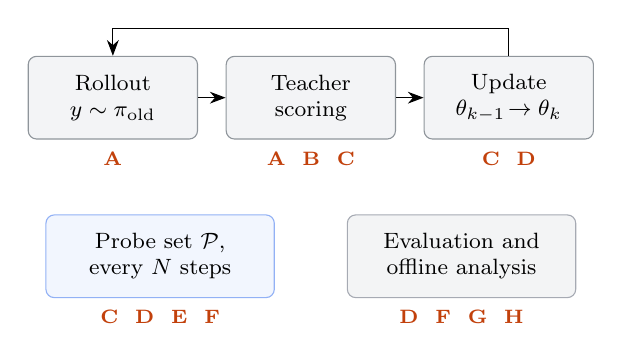
\begin{tikzpicture}[
  stage/.style={draw=ink!50,rounded corners=3pt,fill=soft,align=center,
    font=\footnotesize,minimum width=2.15cm,minimum height=1.05cm},
  grp/.style={font=\scriptsize\bfseries,color=accent,align=center},
  >={Stealth[length=2mm]}]
  \node[stage] (roll) {Rollout\\ $y\sim\piold$};
  \node[stage,right=0.35cm of roll] (score) {Teacher\\ scoring};
  \node[stage,right=0.35cm of score] (upd) {Update\\ $\theta_{k-1}\!\to\theta_k$};
  \draw[->] (roll) -- (score);
  \draw[->] (score) -- (upd);
  \draw[->] (upd.north) -- ++(0,0.35) -| (roll.north);
  \node[grp,below=1pt of roll] {A};
  \node[grp,below=1pt of score] {A\ \ B\ \ C};
  \node[grp,below=1pt of upd] {C\ \ D};
  \node[stage,below=0.95cm of roll,xshift=0.6cm,minimum width=2.9cm,fill=cBlue!6,draw=cBlue!50]
    (probe) {Probe set $\mathcal P$,\\ every $N$ steps};
  \node[stage,below=0.95cm of upd,xshift=-0.6cm,minimum width=2.9cm,fill=cGray!8,draw=cGray!60]
    (eval) {Evaluation and\\ offline analysis};
  \node[grp,below=1pt of probe] {C\ \ D\ \ E\ \ F};
  \node[grp,below=1pt of eval] {D\ \ F\ \ G\ \ H};
\end{tikzpicture}
\end{columns}
\end{frame}

% =====================================================================
\section{A.\quad Sanity Checks}

\begin{frame}{A. Sanity checks (1/2): is the signal computed correctly?}
\begin{stattable}
Empty-$z$ regression & Build the teacher input as in training but without $z$, and score it with $\bar\theta=\theta$. Then $q_t=p_t$, so $\max_t\abs{d_t}$ should stay below the noise floor $\nu$ (next row). & \cFwd\ once & Wrong concatenation, positions shifted by one, chat-template mismatch.\\
Noise floor $\nu$ & Score the same tokens twice under conditions that should not matter (other batch composition; training vs.\ inference engine), giving $q^{(1)}_t,q^{(2)}_t$; $\nu=\pct\abs{\log q^{(1)}_t(y_t)-\log q^{(2)}_t(y_t)}$ over scored tokens. & \cFwd & Values $\abs{d_t}<\nu$ cannot be told apart from numerical noise.\\
Token alignment & Fraction of positions whose token id inside the teacher input equals the sampled $y_t$. & \cFree & Mismatch caused by decoding and re-tokenizing the response.\\
Teacher-input truncation & Distribution of $\abs{x}+\abs{z}+L$; fraction above the teacher context limit $L_{\max}$; fraction in which part of $z$ is cut. & \cFree & The teacher never saw the full $z$.\\
\end{stattable}
\end{frame}

% ---------------------------------------------------------------------
\begin{frame}{A. Sanity checks (2/2): numerics and bookkeeping}
\begin{stattable}
Temperature consistency & The student log-probability must use the sampling temperature $T$ (verl divides the logits by $T$ in \texttt{dp\_actor.py:226}). Choose the teacher's temperature explicitly and log it. & \cFree & A mismatch shifts every $d_t$ systematically.\\
Numerical anomalies & Count of NaN/Inf values; fraction of tokens with $\log p_t(y_t)=0$ exactly or $\log p_t(y_t)<-30$; $\max_t\norm{u_t}_\infty$. & \cFree & Overflow and saturation in bf16.\\
Teacher version & Step at which $\bar\theta$ was last copied from $\theta$. For an EMA teacher $\bar\theta\leftarrow\beta\bar\theta+(1-\beta)\theta$ with decay $\beta\in[0,1)$, also $\norm{\bar\theta-\theta}/\norm{\theta}$. & \cFree & Synchronization works as intended.\\
Duplicated rows & verl-agent pads a batch by copying rows (\texttt{adjust\_batch}, \texttt{multi\_turn\_rollout/utils.py:86}); log the copied fraction. & \cFree & Copies over-weight some responses in both statistics and gradients.\\
\end{stattable}
\vspace{2pt}
\gnote{Line numbers refer to verl-agent at commit 20bd331.}
\end{frame}

% =====================================================================
\section{B.\quad Where the Signal Lands}

\begin{frame}{B. Where the signal lands (1/2): concentration}
\small
Signal mass of a unit: a token has $\abs{d_{i,t}}$, a response $\sum_t\abs{d_{i,t}}$, a prompt $\sum_{i=1}^{G}\sum_t\abs{d_{i,t}}$.
Below, $a_1,\dots,a_n$ are the masses of the $n$ units at one of these levels.\\[3pt]
\begin{stattable}
Gini coefficient & $\mathrm{Gini}=\dfrac{\sum_{j=1}^n\sum_{j'=1}^n\abs{a_j-a_{j'}}}{2n\sum_{j=1}^n a_j}$; 0 means perfectly even, close to 1 means one unit holds almost everything. Report all three levels. & \cFree & Is the update driven by a handful of tokens, responses or prompts?\\
Top-1\% share & $\sum_{j\in\mathcal T}a_j\big/\sum_{j}a_j$, where $\mathcal T$ holds the 1\% of units with the largest $a_j$. & \cFree & The same question, easier to read.\\
Low-signal prompts & Mean signal per token of a prompt $\bar a(x)=\sum_{i,t}\abs{d_{i,t}}\big/\sum_i L_i$; fraction of prompts with $\bar a(x)<\epsilon_{\mathrm{low}}$, a chosen threshold such as $\epsilon_{\mathrm{low}}=\nu$. & \cFree & Like all-correct or all-wrong groups in GRPO: full generation cost, almost no gradient.\\
\end{stattable}
\end{frame}

% ---------------------------------------------------------------------
\begin{frame}{B. Where the signal lands (2/2): per-prompt dynamics}
\small
For a prompt $x$, $k$ runs over the steps at which $x$ is sampled; $\acc_k(x)=\frac1G\sum_{i=1}^G c_i$ is its fraction of correct responses at step $k$; $v_k(x)=\Ind[\acc_k(x)\ge\tfrac12]$ marks it as solved.\\[2pt]
\begin{stattable}
Per-prompt learning curve & First $k$ with $v_k(x)=1$; number of forgetting events $\sum_k\Ind[v_{k-1}(x)=1,\ v_k(x)=0]$ (Toneva et al.\ 2019). & \cFree & Which prompts are learned quickly, and which are learned and then forgotten.\\
Signal vs.\ gain & $\rho_{\mathrm S}$ across prompts between the cumulative signal $\sum_k\bar a_k(x)$ ($\bar a$ at step $k$) and the gain $\acc_{\mathrm{last}}(x)-\acc_{\mathrm{first}}(x)$ (last and first sampled step). & \cFree\newline\cEval & Do prompts that receive more signal improve more?\\
Effective-token fraction & Tokens that enter the loss after masking, divided by all positions of the padded batch tensor. & \cFree & How much compute produces no gradient.\\
Train/eval overlap & Fraction of evaluation prompts that share a 13-token span with some training prompt. & \cOff & Contamination.\\
\end{stattable}
\end{frame}

% =====================================================================
\section{C.\quad Estimator Quality}

\begin{frame}{C. Estimator quality (1/2): single sample vs.\ full distribution}
\begin{columns}[T]
\column{0.49\textwidth}
\textbf{Single-sample estimate} \gnote{(used in training)}
\[
\hat g=\sum_{t=1}^{L}\nabla_\theta\mathcal L_t=-\sum_{t=1}^{L}d_t\,\nabla_\theta\log p_t(y_t)
\]
\column{0.49\textwidth}
\textbf{Full-distribution gradient} \gnote{(needs $q_t$ on all of $\mathcal V$)}
\[
g^{\mathrm{full}}=\sum_{t=1}^{L}\nabla_\theta\KL(p_t\Vert q_t)
\]
\end{columns}
\gnote{By the identity on the training-loss slide, $\E[\hat g-g^{\mathrm{full}}]=0$: the gap is pure noise. Both treat every prefix $h_t$ as fixed, i.e.\ ignore how $\theta$ changes later prefixes.}\par\vspace{4pt}
\begin{stattable}
Direction agreement & $\cos(\hat g,g^{\mathrm{full}})$ per response on $\mathcal P$, and again after averaging over the batch. Restrict to one layer's parameters to keep it cheap. & \cLog\newline\cGrad & How noisy the signal is in gradient space, not just as a scalar.\\
Within-group gradient spread & $\hat g_i$: estimate from response $i$; $\bar g=\frac1G\sum_i\hat g_i$; report $\frac1G\sum_i\norm{\hat g_i-\bar g}^2\big/\norm{\bar g}^2$. & \cGrad & Is $G$ large enough?\\
\end{stattable}
\end{frame}

% ---------------------------------------------------------------------
\begin{frame}{C. Estimator quality (2/2): outcomes and on-policyness}
\begin{stattable}[2.3cm]
Dense signal vs.\ outcome & $\bar d_i=\frac1{L_i}\sum_t d_{i,t}$; report $\AUROC(\bar d\to c)$. & \cFree & Does the per-token judgment agree with final correctness?\\
Sign agreement with GRPO & $\hat A_i=\frac{R_i-\operatorname{mean}(R_1,\dots,R_G)}{\operatorname{std}(R_1,\dots,R_G)+10^{-6}}$, $\mathcal I=\{i:\hat A_i\ne0\}$, pooled over the batch: $\sum_{i\in\mathcal I}\sum_t\Ind[\operatorname{sign}d_{i,t}=\operatorname{sign}\hat A_i]\big/\sum_{i\in\mathcal I}L_i$. & \cFree & With RL mixed in: share of tokens where both signals push the same way.\\
Off-policy ratio & $r_t=\pit(y_t\mid x,h_t)/\piold(y_t\mid x,h_t)$: its percentiles, and the normalized effective sample size over the $n$ tokens of a mini-batch, $\mathrm{ESS}/n=(\sum_t r_t)^2\big/(n\sum_t r_t^2)\in(0,1]$. & \cFree & Drift from on-policy within one step.\\
Staleness & With asynchronous rollout: number of optimizer steps between the parameters that generated a response and the parameters being updated. & \cFree & Does ``on-policy'' still hold? (AsyncOPD, f-OPD)\\
\end{stattable}
\end{frame}

% =====================================================================
\section{D.\quad Gradients and Optimizer}

\begin{frame}{D. Gradients (1/3): gradient noise scale}
\small
$g_b$: gradient averaged over the $b$ sequences of one accumulation step (all data-parallel ranks); $g_B$: gradient averaged over all $B$ sequences of the optimizer step.

If per-sequence gradients have mean $g$ and covariance $\Sigma$, then $\E\norm{g_b}^2=\norm{g}^2+\operatorname{tr}(\Sigma)/b$, likewise for $B$; solving both:
\begin{eqbox}
\[
\widehat{\norm{g}^2}=\frac{B\norm{g_B}^2-b\norm{g_b}^2}{B-b},\qquad
\widehat{\operatorname{tr}\Sigma}=\frac{\norm{g_b}^2-\norm{g_B}^2}{1/b-1/B},\qquad
B_{\mathrm{noise}}=\frac{\widehat{\operatorname{tr}\Sigma}}{\widehat{\norm{g}^2}}
\]
\end{eqbox}
\begin{itemize}
  \item Smooth numerator and denominator separately over steps before dividing.
  \item $B\ll B_{\mathrm{noise}}$: a larger batch still cuts the number of steps almost proportionally; $B\gg B_{\mathrm{noise}}$: extra samples per step are mostly wasted (McCandlish et al.\ 2018).
  \item Cost \cGrad: one extra gradient-norm reduction after the first micro-batch. With token-mean loss aggregation the per-sequence view is approximate.
\end{itemize}
\end{frame}

% ---------------------------------------------------------------------
\begin{frame}{D. Gradients (2/3): step direction and per-token push}
\begin{stattable}
Micro-batch consistency & $g_1,\dots,g_M$: gradients of the $M$ micro-batches of one step, $\bar g_M=\frac1M\sum_m g_m$; report $\frac1M\sum_m\cos(g_m,\bar g_M)$. & \cGrad & Is the step direction stable?\\
Update persistence & $\cos(\Delta\theta_k,\Delta\theta_{k-1})$, per layer (keeping the previous update of every layer may not fit in memory, so pick a few layers). & \cFree & Oscillating, or moving steadily?\\
Per-token logit gradient & $\nabla_{u_t}\mathcal L_t=-d_t\,(e_{y_t}-p_t)$, so $\norm{\nabla_{u_t}\mathcal L_t}=\abs{d_t}\sqrt{1-2p_t(y_t)+\sum_{a}p_t(a)^2}$. Sum it by relative-position bucket $t/L$ and by token type (digits, formula symbols, format tokens, words such as ``wait''). & \cLog\ \gnote{(the actor already has the logits)} & Where parameters are actually pushed: a confident token ($p_t(y_t)\to1$) gets almost no gradient even when $\abs{d_t}$ is large.\\
\end{stattable}
\vspace{2pt}
\gnote{Ignores clipping and the token-aggregation weight of the loss, which only rescale or zero some rows.}
\end{frame}

% ---------------------------------------------------------------------
\begin{frame}{D. Gradients (3/3): landscape and plasticity}
\begin{stattable}
Sharpness & $\lambda_{\max}$: largest eigenvalue of $\nabla^2_\theta\mathcal L_{\mathcal P}$, where $\mathcal L_{\mathcal P}$ is the sum of $\mathcal L_t$ over all tokens of $\mathcal P$; power iteration with Hessian--vector products (PyHessian). & \cOff & Is training moving into sharper regions?\\
Effective rank of features & $\sigma_1,\dots,\sigma_r$: singular values of $\Phi_\ell$; $\bar\sigma_j=\sigma_j/\sum_{j'}\sigma_{j'}$; $\operatorname{erank}(\Phi_\ell)=\exp\!\big(-\sum_j\bar\sigma_j\log\bar\sigma_j\big)$ (Roy \& Vetterli 2007). & \cFwd & Collapsing features, a known correlate of lost plasticity.\\
Weight-norm growth & $\norm{\theta_k}/\norm{\theta_0}$, per layer. & \cFree & Weight growth also accompanies lost plasticity (Dohare et al.\ 2024).\\
Dormant units & Fraction of MLP units (inputs of the down-projection) whose absolute activation stays below a threshold $\delta$ on every probe token. & \cFwd & Units that stopped contributing.\\
\end{stattable}
\end{frame}

% =====================================================================
\section{E.\quad Calibration and Confidence}

\begin{frame}{E. Calibration (1/2): confidence scores and how to grade them}
\small
Reverse KL is mode-seeking (Gu et al.\ 2024), so distilled students tend to become over-confident. Two confidence scores per response:\vspace{-4pt}
\[
\kappa^{\mathrm{tok}}_i=\exp\Big(\frac1{\abs{\mathcal S_i}}\sum_{t\in\mathcal S_i}\log p_{i,t}\big(y^{(i)}_t\big)\Big),\qquad
\kappa^{\mathrm{vote}}_i=\frac1G\sum_{j=1}^{G}\Ind\big[\ans(y^{(j)})=\ans(y^{(i)})\big]
\]
\gnote{$\kappa^{\mathrm{tok}}_i$: geometric-mean probability of the answer tokens. $\kappa^{\mathrm{vote}}_i$: share of the group with the same final answer.}\\
For $n$ responses with scores $\kappa_i$ (either kind) and verdicts $c_i$:\vspace{-2pt}
\begin{columns}[T]
\column{0.56\textwidth}
\begin{eqbox}
\[
\mathrm{ECE}=\sum_{m=1}^{N_{\mathrm{bin}}}\frac{\abs{\mathcal B_m}}{n}\,\Big|\operatorname*{mean}_{i\in\mathcal B_m}c_i-\operatorname*{mean}_{i\in\mathcal B_m}\kappa_i\Big|
\]
\end{eqbox}
\gnote{$[0,1]$ is split into $N_{\mathrm{bin}}$ equal bins; $\mathcal B_m$ = responses whose $\kappa_i$ falls in bin $m$ (Guo et al.\ 2017).}
\column{0.40\textwidth}
\begin{eqbox}
\[
\mathrm{Brier}=\frac1n\sum_{i=1}^n(\kappa_i-c_i)^2
\]
\end{eqbox}
Discrimination: $\AUROC(\kappa\to c)$.\\
All three: \cFree
\end{columns}
\end{frame}

% ---------------------------------------------------------------------
\begin{frame}{E. Calibration (2/2): over-confidence and uncertainty}
\begin{stattable}
Wrong-answer confidence & $\operatorname{mean}\{\kappa_i: c_i=0\}$. & \cFree & Is over-confidence getting worse?\\
Self-certainty & $\frac1{L_i}\sum_t\KL(U\Vert p_{i,t})$, where $U$ is the uniform distribution on $\mathcal V$ (Kang et al.\ 2025). & \cLog & Overall confidence level, read from the whole distribution.\\
Semantic entropy & Cluster the $G$ responses by final answer; a cluster $\mathcal C$ has share $\hat p_{\mathcal C}=\abs{\mathcal C}/G$; $\mathrm{SE}(x)=-\sum_{\mathcal C}\hat p_{\mathcal C}\log\hat p_{\mathcal C}$. Report $\AUROC(-\mathrm{SE}\to c^{\mathrm{maj}})$, with $c^{\mathrm{maj}}(x)=1$ if the largest cluster is correct. & \cFree & Does uncertainty still flag errors? (Simplified from Kuhn et al.\ 2023, which clusters by entailment.)\\
Hedging frequency & Occurrences of phrases such as ``I'm not sure'' or ``might be'', per 1000 tokens. & \cFree & Has the model stopped expressing doubt?\\
\end{stattable}
\end{frame}

% =====================================================================
\section{F.\quad Representations and Mechanisms}

\begin{frame}{F. Representations (1/2): how much, and where, the network changed}
\small
Linear CKA (centered kernel alignment) of two matrices $X$ and $Y$ with the same $n$ rows (same tokens in the same order) and centered columns (Kornblith et al.\ 2019):
\begin{eqbox}
\[
\mathrm{CKA}(X,Y)=\frac{\norm{Y^\top X}_F^2}{\norm{X^\top X}_F\,\norm{Y^\top Y}_F}\in[0,1]
\]
\end{eqbox}
\begin{stattable}
Layer-wise drift & $\mathrm{CKA}\big(\Phi_\ell\text{ under }\theta_0,\ \Phi_\ell\text{ under }\theta_k\big)$ for every layer $\ell$, on the same probe tokens. & \cFwd & Are the changes in shallow or deep layers?\\
Teacher--student alignment & Rows are response positions $t$. $X$: student states at layer $\ell$ given $(x,h_t)$; $Y$: teacher states at layer $\ell$ given $(x,z,h_t)$. Plot over training. & \cFwd\ \gnote{(hook the teacher pass)} & Is the student's internal state moving toward what $z$ induces in the teacher?\\
\end{stattable}
\end{frame}

% ---------------------------------------------------------------------
\begin{frame}{F. Representations (2/2): mechanisms}
\begin{stattable}
Attention mass on $z$ & $\mathcal Z$: positions of $z$ in the teacher input; $\mathcal R$: response positions; $\omega^{(\ell,j)}_{t,s}$: attention weight from position $t$ to $s$ in head $j$ of layer $\ell$; $N_h$ heads per layer. $\alpha_\ell=\frac{1}{\abs{\mathcal R}N_h}\sum_{t\in\mathcal R}\sum_{j=1}^{N_h}\sum_{s\in\mathcal Z}\omega^{(\ell,j)}_{t,s}$. & \cFwd & How much the teacher reads $z$; with $\bar\theta=\theta$, whether this changes in training.\\
Logit-lens settling layer & $W_U$: unembedding matrix; $\operatorname{Norm}$: final normalization. $\ell^\star_t$: smallest $\ell$ such that $\arg\max_a[W_U\operatorname{Norm}(\phi^{(\ell')}_t)]_a=\arg\max_a p_t(a)$ for every $\ell'\ge\ell$. & \cFwd & Does training move decisions to earlier layers?\\
Correctness probe & Logistic regression from $\phi^{(\ell)}_{L_i}$ (last response token) to $c_i$; held-out AUROC for each layer $\ell$. & \cOff & Does the model ``know'' it is wrong?\\
Activation magnitude & $\max_{t,\ell}\norm{\phi^{(\ell)}_t}_\infty$ and $\max_t\norm{u_t}_\infty$. & \cFwd & bf16 risk (massive activations, Sun et al.\ 2024).\\
\end{stattable}
\vspace{1pt}
\gnote{FlashAttention kernels do not return attention weights, hence eager attention for $\alpha_\ell$.}
\end{frame}

% =====================================================================
\section{G.\quad Generalization, Forgetting, Robustness}

\begin{frame}{G. Generalization (1/2): what else changed}
\begin{stattable}
General-capability regression & Before vs.\ after training on suites such as MMLU-Pro, GPQA, IFEval, HumanEval (or the suites that matter to you). & \cEval & Were other skills paid for the gain?\\
Memorization gap & $\acc(\mathcal D_{\mathrm{train}})-\acc(\mathcal D_{\mathrm{held}})$. & \cEval & Learning methods, or memorizing items?\\
Cross-domain transfer & Train on math; evaluate on code, science, logic. & \cEval & How far does the gain transfer?\\
Paraphrase robustness & Write each evaluation prompt in $J$ templates or paraphrases; $\acc_j$: accuracy under template $j$; report $\operatorname{std}(\acc_1,\dots,\acc_J)$. & \cEval & Over-fitted to the training template?\\
\end{stattable}
\end{frame}

% ---------------------------------------------------------------------
\begin{frame}{G. Generalization (2/2): harder inputs, facts, imperfect references}
\begin{stattable}
Difficulty extrapolation & Accuracy on problems harder than the training set (higher difficulty levels, competition sets). & \cEval & Does the gain extend to harder problems?\\
Factuality & On SimpleQA-style sets: fraction of attempted answers that are wrong. & \cEval & Does over-confidence spill over into factual questions?\\
Noisy-$z$ robustness & Train with a fraction $\eta$ of the $z$ replaced by wrong references; plot final $\acc(\mathcal D_{\mathrm{held}})$ against $\eta$. & \cRun & Sensitivity to reference quality; real datasets contain wrong solutions.\\
\end{stattable}
\end{frame}

% =====================================================================
\section{H.\quad Experimental Rigor}

\begin{frame}{H. Rigor (1/2): uncertainty of the headline numbers}
\begin{itemize}
  \item \textbf{Seeds.} At least 3 training seeds per setting; report the mean and a 95\% confidence interval (Agarwal et al.\ 2021).
  \item \textbf{Bootstrap over problems.} Resample problems with replacement, recompute the metric, take the 2.5th and 97.5th percentiles. On a 30-problem set one problem is $1/30\approx3.3$ points, so use avg@16 or more.
  \item \textbf{Paired comparison} of methods A and B on the same problems.
\end{itemize}
\begin{columns}[T]
\column{0.52\textwidth}
\begin{eqbox}
\[
\chi^2=\frac{(n_{01}-n_{10})^2}{n_{01}+n_{10}}
\]
\end{eqbox}
\column{0.44\textwidth}
\small
$n_{10}$: problems A solves and B does not; $n_{01}$: the reverse. Compare with the $\chi^2$ distribution with 1 degree of freedom (McNemar 1947).
\end{columns}
\vspace{4pt}
\gnote{With avg@16 the per-problem score is not binary; then use a paired bootstrap on per-problem differences instead.}
\end{frame}

% ---------------------------------------------------------------------
\begin{frame}{H. Rigor (2/2): noise floors, compute, checkpoint choice}
\begin{itemize}
  \item \textbf{Noise floor of probe statistics.} Run $\mathcal P$ twice on the same checkpoint with different sampling seeds, giving values $\hat m^{(1)},\hat m^{(2)}$ of a statistic. Changes smaller than $\abs{\hat m^{(1)}-\hat m^{(2)}}$ should not be interpreted.
  \item \textbf{Compute-matched axes.} Besides training steps, plot against cumulative generated tokens, teacher-scored tokens and GPU-hours. OPSD adds a teacher forward pass to every step, so per-step plots flatter it.
  \item \textbf{Fixed checkpoint selection.} Report the final checkpoint, plus the best one chosen by a rule fixed in advance on a validation split. Never select on the test set.
\end{itemize}
\end{frame}

% =====================================================================
\section{Putting It Together}

\begin{frame}{Schedule: three tiers}
\scriptsize
\setlength{\tabcolsep}{4pt}\renewcommand{\arraystretch}{1.15}
\begin{tabularx}{\linewidth}{@{}>{\bfseries}l >{\raggedright\arraybackslash}p{2.4cm} Y@{}}
\toprule
Tier & When / data & Statistics\\
\midrule
1 & every step, full training batch & A: token alignment, truncation, temperature, numerics, teacher version, duplicated rows.
B: all except train/eval overlap. C: dense vs.\ outcome, sign agreement, off-policy ratio, staleness.
D: noise scale, micro-batch consistency, update persistence, per-token logit gradient, weight norm.
E: confidence scores, ECE, Brier, wrong-answer confidence, semantic entropy, hedging.\\
2 & every $N$ steps, probe set $\mathcal P$ & C: direction agreement, within-group gradient spread. D: effective rank, dormant units.
E: self-certainty. F: drift, teacher--student alignment, attention mass on $z$, logit lens, activation magnitude.\\
3 & checkpoints and dumps & A: empty-$z$ regression and noise floor (once). B: train/eval overlap. D: sharpness. F: correctness probe. G and H.\\
\bottomrule
\end{tabularx}
\vspace{4pt}
\begin{alertblock}{Compute tier-1 group statistics on the driver}
\footnotesize Per-prompt and per-verdict statistics need the whole batch, but in verl each data-parallel worker sees only a shard.
\end{alertblock}
\end{frame}

% ---------------------------------------------------------------------
\begin{frame}{What to dump at each probe point}
\small Saving raw quantities lets every statistic above be computed offline, and new ones be added later without retraining.
\begin{columns}[T]
\column{0.5\textwidth}
\begin{block}{Per token}
\footnotesize
token id, position $t$, response index $i$\\
$\log p_{i,t}(y^{(i)}_t)$, \ $\log q_{i,t}(y^{(i)}_t)$, \ $\norm{\nabla_{u_t}\mathcal L_t}$\\
the 20 most likely tokens and their probabilities under $p_{i,t}$ and under $q_{i,t}$
\end{block}
\begin{block}{Per response}
\footnotesize
$c_i$, \ $L_i$, \ $\ans(y^{(i)})$, \ $\kappa^{\mathrm{tok}}_i$, \ $\kappa^{\mathrm{vote}}_i$
\end{block}
\column{0.46\textwidth}
\begin{block}{Selected layers, sampled positions}
\footnotesize
$\phi^{(\ell)}_t$ in bf16: $2\dm$ bytes per token per layer.
\end{block}
\begin{exampleblock}{Size estimate}
\footnotesize
Two top-20 lists, 4-byte id + 2-byte probability: $2\times20\times6=240$ bytes per token.\\[2pt]
Hidden states, $\dm=1536$ (Qwen2.5-1.5B): about 3\,KB per token per layer, so 3\,GB per layer for $10^6$ tokens. Subsample positions.
\end{exampleblock}
\end{columns}
\end{frame}

% ---------------------------------------------------------------------
\begin{frame}{Priorities for Part I}
\begin{enumerate}
  \setlength\itemsep{6pt}
  \item \textbf{All of A.} Almost free, and if any check fails, no other statistic means anything.
  \item \textbf{From H: several seeds and compute-matched axes.} Reviewers usually ask for both.
  \item \textbf{G: general-capability regression, and E: wrong-answer confidence.} Forgetting and over-confidence are the two most common side effects of distillation.
  \item \textbf{The \cFree{} rows of B, C and E} go into tier 1; \textbf{D and F} go into tier 2 on the probe set.
\end{enumerate}
\end{frame}

% =====================================================================
%                              PART II
% =====================================================================
\begin{frame}[standout]
Part II\\[6pt]
{\normalsize Statistics for one hypothesis:\\ privileged-information PMI and prefix compatibility (idea 003)}
\end{frame}

\section{II.0\quad Notation and Hypotheses}

\begin{frame}{Part II notation (1/3): decomposing the signal}
Teacher network \emph{without} $z$, with the same prompt template as the student:\ \ $q^0_t=\pitea(\cdot\mid x,h_t)$.
\begin{eqbox}
\[
d_t=\underbrace{\log q_t(y_t)-\log q^0_t(y_t)}_{\mathrm{PMI}_t}
+\underbrace{\log q^0_t(y_t)-\log p_t(y_t)}_{\Delta^{\mathrm{snap}}_t}
\]
\end{eqbox}
\begin{itemize}
  \setlength\itemsep{3pt}
  \item $\mathrm{PMI}_t$ (named after pointwise mutual information): how much seeing $z$ raises the teacher's log-probability of $y_t$.
  \item $\Delta^{\mathrm{snap}}_t$ (snapshot gap): the gap between teacher and student parameters.
  \item If $\bar\theta$ is set to $\theta$ at rollout time, $\Delta^{\mathrm{snap}}_t=0$ on the first mini-batch of a step, so $d_t=\mathrm{PMI}_t$ there and $\mathrm{PMI}_t$ costs nothing extra. On later mini-batches $\Delta^{\mathrm{snap}}_t=-\log r_t$ ($r_t$ from Section C).
\end{itemize}
\end{frame}

% ---------------------------------------------------------------------
\begin{frame}{Part II notation (2/3): prefix compatibility}
For any policy $\pi$, the probability of a prefix is $\pi(h_t\mid x)=\prod_{u=1}^{t-1}\pi(y_u\mid x,h_u)$, and likewise with $z$ in the context. By the chain rule:
\begin{eqbox}
\[
S_t=\sum_{u=1}^{t-1}\mathrm{PMI}_u=\log\frac{\pitea(h_t\mid x,z)}{\pitea(h_t\mid x)},\qquad S_1=0
\]
\end{eqbox}
\begin{itemize}
  \setlength\itemsep{3pt}
  \item $S_t>0$: the prefix is more likely when $z$ is visible; it follows $z$'s route.
  \item $S_t<0$: the prefix has left that route, e.g.\ a different method or an error.
  \item $S_t\approx0$: no evidence yet, typical early in the response.
\end{itemize}
\end{frame}

% ---------------------------------------------------------------------
\begin{frame}{Part II notation (3/3): further symbols}
\begin{symtable}
$\mathcal H(p)=-\sum_{a}p(a)\log p(a)$ & entropy of a distribution $p$ over $\mathcal V$\\
$\mathrm p_{1},\ \mathrm p_{5},\ \mathrm p_{10},\ \mathrm p_{50},\ \dots$ & percentiles, defined like $\pct$\\
$\operatorname{Var}$, $\operatorname{Cov}$, $\operatorname{corr}$ & variance, covariance, Pearson correlation over tokens\\
$T_m(p)$;\ \ $\operatorname{rank}_p(a)$ & the $m$ most likely tokens; one plus the count of more likely tokens\\
$\hat y_t=\arg\max_a q_t(a)$;\ \ $\mathrm{eos}$ & teacher's top-1 token at $t$; end-of-sequence token\\
$\mathcal W$ & reflection words: wait, but, hmm, let me check, actually, alternatively\\
$z^+$;\ \ $z^-$ & correct reference ($z^+=z$); a wrong one in the same template\\
$\pi(y\mid x)$,\ \ $\pi(y\mid x,z)$ & $\prod_{t=1}^{L}\pi(y_t\mid x,h_t)$: whole-response probability (same with $z$)\\
\end{symtable}
\end{frame}

% ---------------------------------------------------------------------
\begin{frame}{Part II: hypotheses to test (none tested yet)}
\small
\begin{itemize}
  \setlength\itemsep{1pt}
  \item \textbf{H1 (derivability).} OPSD helps when the student could derive $z$ itself (e.g.\ an image crop). On long reasoning it hurts when the student cannot derive $z$ (e.g.\ a reference solution), more so the more information $z$ carries.
  \item \textbf{H2 (compatibility, not position).} Whether the teacher's guidance at $t$ helps depends on $S_t$, not on the relative position $t/L$.
  \item \textbf{H3 (reflection tokens).} Tokens from $\mathcal W$ get negative $\mathrm{PMI}_t$ where $S_t\ge0$, and near-zero or positive $\mathrm{PMI}_t$ where $S_t<0$.
\end{itemize}
\footnotesize
\setlength{\tabcolsep}{4pt}\renewcommand{\arraystretch}{1.1}
\begin{tabularx}{\linewidth}{@{}>{\bfseries}l Y@{}}
\toprule
Hypothesis & Key statistics\\
\midrule
H1 & $\mathrm{PMI}_t$ by type of $z$ (II.4); reflection-word rate (II.6); accuracy vs.\ generation budget (II.1)\\
H2 & reliability AUROC, incremental value, position-stratified AUROC, help vs.\ compatibility (II.5)\\
H3 & $\mathrm{PMI}_t$ of reflection words, split by the sign of $S_t$ and by verdict (II.4)\\
\bottomrule
\end{tabularx}
\end{frame}

% =====================================================================
\section{II.1\quad Training Health and Task Metrics}

\begin{frame}{II.1 Training health (1/2): is the run stable?}
\begin{stattable}
Loss and gradient norm & Loss; gradient norm before clipping; fraction of steps skipped because of non-finite gradients. & \cFree & Is training stable?\\
Clip fraction, approximate KL & $\epsilon_{\mathrm{clip}}$: PPO clip range. Fraction of tokens with $r_t\notin[1-\epsilon_{\mathrm{clip}},1+\epsilon_{\mathrm{clip}}]$; mean of $\log\piold(y_t\mid x,h_t)-\log\pit(y_t\mid x,h_t)$ (verl: \texttt{pg\_clipfrac}, \texttt{ppo\_kl}). & \cFree & How far one step moves the policy.\\
Student entropy & $\mathcal H(p_t)$: mean, $\mathrm p_{10}$, $\mathrm p_{50}$, $\mathrm p_{90}$, and the fraction of tokens with $\mathcal H(p_t)<0.01$. & \cFree & Entropy collapse?\\
\end{stattable}
\end{frame}

% ---------------------------------------------------------------------
\begin{frame}{II.1 Training health (2/2): outputs and engines}
\begin{stattable}
Length and truncation & $L$: mean, $\mathrm p_{50}$, $\mathrm p_{90}$, max; fraction of responses cut at the generation limit before $\mathrm{eos}$. & \cFree & Does OPSD lengthen or shorten answers? Is the budget enough?\\
Degenerate output & Fraction of responses with a repeating loop, a format violation (e.g.\ no \texttt{\textbackslash boxed\{\}}), or mixed languages. & \cFree & Is the output degenerating?\\
Engine mismatch & $\pi_{\mathrm{inf}}$: probabilities reported by the inference engine while sampling. Max and $\pct$ of $\abs{\log\pi_{\mathrm{inf}}(y_t\mid x,h_t)-\log\piold(y_t\mid x,h_t)}$ (\texttt{ray\_trainer.py:1153}). & \cFree & Hidden off-policyness.\\
\end{stattable}
\end{frame}

% ---------------------------------------------------------------------
\begin{frame}{II.1 Task metrics (1/2): accuracy and exploration}
\begin{stattable}
Online accuracy & Mean of $c_i$ on the training batch, logged even when $c_i$ is not part of the loss. & \cFree & Is the student improving?\\
pass@$K$ curve & $K$: number of attempts. For a problem with $n_{\mathrm{smp}}$ samples, $n_{\mathrm{cor}}$ of them correct: $\text{pass@}K=1-\binom{n_{\mathrm{smp}}-n_{\mathrm{cor}}}{K}\big/\binom{n_{\mathrm{smp}}}{K}$ (Chen et al.\ 2021), averaged over problems, for $K=1,2,4,\dots,64$. & \cEval & Does distillation narrow what the student can find?\\
maj@$K$ & Fraction of problems whose most frequent answer among $K$ samples is correct. & \cEval & Accuracy with voting.\\
Exploration gap & pass@64 minus pass@1. & \cEval & Is diversity being compressed?\\
Difficulty buckets & $\acc_{\theta_0}(x)$: fraction of correct samples for $x$ under $\theta_0$. Buckets $\{0\}$, $(0,\tfrac12]$, $(\tfrac12,1)$, $\{1\}$; accuracy per bucket over training. & \cEval & Which problems gain, which lose?\\
\end{stattable}
\end{frame}

% ---------------------------------------------------------------------
\begin{frame}{II.1 Task metrics (2/2): regressions, ceiling, budget}
\begin{stattable}
Per-problem flips & A problem is solved if at least half of its samples are correct. Between $\theta_0$ and the final checkpoint: counts of unsolved$\to$solved, solved$\to$unsolved, always unsolved, always solved. & \cEval & Are some problems getting worse?\\
Imitation gap & $\acc$ of the teacher answering with $z$ in context (sampling from $\pitea(\cdot\mid x,z)$) minus $\acc$ of the student. & \cEval & How far could the teacher lift the student?\\
Accuracy vs.\ budget & $\acc(\mathcal D_{\mathrm{held}})$ at several generation limits. & \cEval & Does a longer budget hurt? (reported by Rethinking OPSD)\\
Length by verdict & Mean $L_i$ over responses with $c_i=1$ and with $c_i=0$, separately. & \cFree & How length relates to correctness.\\
\end{stattable}
\vspace{2pt}
\gnote{Out-of-domain accuracy is covered by Part I, Section G.}
\end{frame}

% =====================================================================
\section{II.2\quad The Signal $d_t$}

\begin{frame}{II.2 The signal $d_t$ (1/2): distribution}
\begin{stattable}
Shape & Mean $\mu_d$, standard deviation $\sigma_d$, $\mathrm p_{1}$, $\mathrm p_{5}$, $\mathrm p_{50}$, $\mathrm p_{95}$, $\pct$, min, max, kurtosis $\E[(d_t-\mu_d)^4]/\sigma_d^4$. & \cFree & Is the signal heavy-tailed?\\
Sign and tails & $\Pr(d_t>0)$, $\Pr(d_t<-5)$, $\Pr(\abs{d_t}>2)$. & \cFree & Mostly pushing tokens up, or down?\\
Near-zero share & $\Pr(\abs{d_t}<\epsilon_{\mathrm{low}})$, with $\epsilon_{\mathrm{low}}$ from Section B. & \cFree & How many tokens get almost no supervision?\\
Response-level & $\sum_t d_{i,t}$, $\bar d_i$, and the variance of $d_{i,t}$ within a response. & \cFree & How much responses differ.\\
\end{stattable}
\end{frame}

% ---------------------------------------------------------------------
\begin{frame}{II.2 The signal $d_t$ (2/2): where it falls}
\begin{stattable}
Position buckets & Split $t/L$ into 10 equal buckets; mean and variance of $d_t$ per bucket. & \cFree & Position effect; PW-OPSD and LGR reach opposite conclusions.\\
By verdict & Mean $d_{i,t}$ over responses with $c_i=1$ and with $c_i=0$. & \cFree & Does the teacher keep rewriting answers that are already correct?\\
End-of-sequence signal & $\log q_t(\mathrm{eos})-\log p_t(\mathrm{eos})$ at every position. & \cLog & Is a length change caused by the teacher pushing to stop earlier or later?\\
Token categories & Mean $d_t$ for tokens in $\mathcal W$, digits, formula symbols, format tokens, and answer tokens ($t\in\mathcal S_i$). & \cFree & Which kinds of token carry the signal?\\
\end{stattable}
\end{frame}

% =====================================================================
\section{II.3\quad Teacher--Student Distribution Gap}

\begin{frame}{II.3 Distribution gap (1/2): how far apart are $p_t$ and $q_t$?}
\begin{stattable}
Per-token divergences & $\KL(p_t\Vert q_t)$, $\KL(q_t\Vert p_t)$; $\mathrm{JSD}=\frac12\KL(p_t\Vert m_t)+\frac12\KL(q_t\Vert m_t)$ with $m_t=\frac12(p_t+q_t)$; $\mathrm{TV}=\frac12\sum_a\abs{p_t(a)-q_t(a)}$. & \cLog & Size of the gap; how much switching between forward and reverse KL would matter.\\
Top-1 agreement & $\Pr\big[\arg\max_a p_t(a)=\hat y_t\big]$. & \cLog & Do both want the same next token?\\
Teacher's view of the sample & $q_t(y_t)$ and $\operatorname{rank}_{q_t}(y_t)$. & \cFree\newline\cLog & Does the student often write tokens the teacher finds implausible?\\
Top-10 overlap & $\abs{T_{10}(p_t)\cap T_{10}(q_t)}\big/\abs{T_{10}(p_t)\cup T_{10}(q_t)}$. & \cLog & How similar are the candidate sets?\\
\end{stattable}
\end{frame}

% ---------------------------------------------------------------------
\begin{frame}{II.3 Distribution gap (2/2): entropy and approximation error}
\begin{stattable}
Teacher entropy & $\mathcal H(q_t)$, and the 2-D histogram of $(\mathcal H(p_t),\mathcal H(q_t))$. & \cLog & Where the teacher is sure and the student hesitates (SEAD partitions tokens this way).\\
Top-$m$ mass & $\sum_{a\in T_m(q_t)}q_t(a)$ for the $m$ kept by a truncated loss. & \cLog & Mass ignored by a top-$m$ approximation of the KL.\\
Single sample vs.\ exact & $-d_t$ is an unbiased estimate of $\KL(p_t\Vert q_t)$; report $\operatorname{corr}(-d_t,\KL(p_t\Vert q_t))$. & \cLog & Noise of the single-sample signal (vOPD); the gradient-level version is in Section C.\\
\end{stattable}
\end{frame}

% =====================================================================
\section{II.4\quad PMI Decomposition and Prefix Compatibility}

\begin{frame}{II.4 Identity checks: run before anything else}
\small
On about 20 responses, before trusting any statistic in this part:
\begin{enumerate}
  \setlength\itemsep{4pt}
  \item \textbf{Sum identity.} Check
  \[
  \sum_{t=1}^{L}\mathrm{PMI}_t=\log\pitea(y\mid x,z)-\log\pitea(y\mid x)
  \]
  with whole-response log-probabilities computed separately; the error per token should be below $10^{-3}$.
  \item \textbf{Same tokens.} The response token ids are identical in the two prompt templates (with and without $z$).
  \item \textbf{Logged signal.} With $\bar\theta$ synchronized to $\theta$, the $d_t$ logged during training equals $\mathrm{PMI}_t$ recomputed offline.
\end{enumerate}
\gnote{Cost: \cFwd{} once. These complement the general sanity checks of Section A.}
\end{frame}

% ---------------------------------------------------------------------
\begin{frame}{II.4 Per-token features (idea 003, F0--F7)}
\scriptsize
\setlength{\tabcolsep}{4pt}\renewcommand{\arraystretch}{1.12}
\begin{tabularx}{\linewidth}{@{}>{\bfseries}l >{\raggedright\arraybackslash}p{3.3cm} Y >{\centering\arraybackslash}p{1.6cm}@{}}
\toprule
ID & Feature & Definition & Cost\\
\midrule
F0 & relative position (baseline) & $(t-0.5)/L$ & \cFree\\
F1 & teacher entropy (baseline) & $\mathcal H$ of $q_t$ restricted to $T_{16}(q_t)$, renormalized (PW-OPSD) & \cLog\\
F2 & PMI & $\mathrm{PMI}_t$ & \cFree{} / \cFwd\\
F3 & cumulative PMI & $S_t$ & as F2\\
F4 & mean cumulative PMI & $S_t/(t-1)$ for $t\ge2$ & as F2\\
F5 & local privileged divergence & $\KL(q_t\Vert q^0_t)$ on $T_{64}(q_t)\cup T_{64}(q^0_t)$ plus one bucket for the rest & \cLog\\
F6 & candidate PMI & $\log q_t(a)-\log q^0_t(a)$ for $a\in T_3(q_t)$: max and mean & \cLog\\
F7 & contrastive cumulative PMI & $\sum_{u=1}^{t-1}\big[\log\pitea(y_u\mid x,z^+,h_u)-\log\pitea(y_u\mid x,z^-,h_u)\big]$ & \cFwd\\
\bottomrule
\end{tabularx}
\vspace{2pt}
\gnote{F2--F4 are \cFree{} when $\bar\theta=\theta$. F7 separates the content of $z$ from reference style. II.5 tests F0--F7 as reliability predictors.}
\end{frame}

% ---------------------------------------------------------------------
\begin{frame}{II.4 PMI statistics during training (1/2)}
\gnote{Here and on the next slide, \cFree{} applies when $\bar\theta=\theta$, \cFwd{} otherwise.}\par\vspace{1pt}
\begin{stattable}
PMI distribution & Distribution of $\mathrm{PMI}_t$, overall and by position bucket and token category. & \cFree\newline\cFwd & Which tokens does $z$ favor or penalize?\\
Variance decomposition & $\operatorname{Var}(d_t)=\operatorname{Var}(\mathrm{PMI}_t)+\operatorname{Var}(\Delta^{\mathrm{snap}}_t)+2\operatorname{Cov}(\mathrm{PMI}_t,\Delta^{\mathrm{snap}}_t)$. & \cFwd & With a frozen or EMA teacher, which part drives $d_t$?\\
Compatibility profile & Percentiles of $S_t$ against $t$; fraction of tokens with $S_t<0$; distribution of $S_{L+1}$ on correct and on wrong responses. & \cFree\newline\cFwd & Are prefixes following $z$'s route?\\
Compatibility vs.\ signal & $\operatorname{corr}(S_t,\abs{d_t})$. & \cFree\newline\cFwd & Is the signal more extreme on incompatible prefixes?\\
\end{stattable}
\end{frame}

% ---------------------------------------------------------------------
\begin{frame}{II.4 PMI statistics during training (2/2)}
\begin{stattable}
Reflection-word PMI (H3) & Mean $\mathrm{PMI}_t$ where $y_t\in\mathcal W$: correct vs.\ wrong responses; within wrong ones, $S_t\ge0$ vs.\ $S_t<0$. Control: position-matched tokens not in $\mathcal W$. & \cFree\newline\cFwd & Does suppression depend on the prefix state?\\
Contrastive PMI & $\log\pitea(y_t\mid x,z^+,h_t)-\log\pitea(y_t\mid x,z^-,h_t)$. & \cFwd & Content effect without reference style (RLCSD).\\
PMI by type of $z$ & Same statistics with $z$ = final answer only, full solution, or a hint. & \cFwd{} per type & More information, more harm? (H1)\\
Sequence level & With $\bar\theta=\theta$: $\E_{y\sim\pit(\cdot\mid x)}[S_{L+1}]=-\KL\big(\pit(\cdot\mid x)\,\Vert\,\pit(\cdot\mid x,z)\big)$. & \cFree & Is training pulling $\pit(\cdot\mid x)$ toward $\pit(\cdot\mid x,z)$?\\
\end{stattable}
\end{frame}

% =====================================================================
\section{II.5\quad Prefix Reliability: Branch Continuations}

\begin{frame}{II.5 Branch labels: when does following the teacher help?}
\small
\textbf{Spine}: a fixed student response (correct: $c=1$; wrong: $c=0$). $h\oplus a$: prefix $h$ followed by token $a$. $\hat V(h)$: fraction of $n_{\mathrm{roll}}$ student continuations from $h$, without $z$, that are correct.
\begin{columns}[T]
\column{0.49\textwidth}
\begin{block}{Correct spines (PW-OPSD protocol)}
\footnotesize
Up to 5 positions per problem with the highest F1; force each $a\in T_3(q_t)$; $n_{\mathrm{roll}}=6$.\\
\textbf{diversity}: at least two candidates reach $\hat V(h_t\oplus a)\ge0.75$.\\
\textbf{real-uncertain}: all candidates, and their mean, below $0.40$.\\
Otherwise \textbf{gray}, excluded from AUROC.
\end{block}
\column{0.47\textwidth}
\begin{block}{Wrong spines (help label)}
\footnotesize
5 positions per spine, spread evenly over $t/L$; $n_{\mathrm{roll}}=8$:
\[
\Delta_t=\hat V(h_t\oplus\hat y_t)-\hat V(h_t\oplus y_t)
\]
$\Delta_t>0$: the teacher's top-1 token helps a student without $z$. If $\hat y_t=y_t$, set $\Delta_t=0$ and report how often this happens.
\end{block}
\end{columns}
\vspace{2pt}
\gnote{Cost \cBr: problems $\times5\times3\times6$ continuations for correct spines, problems $\times5\times2\times8$ for wrong spines.}
\end{frame}

% ---------------------------------------------------------------------
\begin{frame}{II.5 Statistics on the branch labels}
\begin{stattable}
Reliability AUROC & AUROC of each of F0--F7 for real-uncertain vs.\ diversity, after subtracting each problem's mean score; problem-level bootstrap 95\% CI (2000 resamples). & \cBr & Can compatibility beat position?\\
Incremental value & 5-fold logistic regression, folds split by problem: held-out AUROC of F0 plus one feature minus that of F0 alone, with bootstrap CI. & \cOff & Information beyond position.\\
Position-stratified AUROC & AUROC of F3 and F5 within each third of $t/L$. & \cOff & Separates compatibility from its correlation with position.\\
Help vs.\ compatibility & $\rho_{\mathrm S}(\Delta_t,S_t)$; partial correlation given $t/L$ (of residuals after regressing both on $t/L$); mean $\Delta_t$ for $S_t\ge0$ vs.\ $S_t<0$. & \cBr & Does leaving $z$'s route distort guidance (LGR)?\\
Rescue and endorsement & Rescue: mean $\hat V(h_t\oplus\hat y_t)$ where $\hat V(h_t)\le0.1$. Error step: $\hat V(h_{t+1})\le\hat V(h_t)-0.3$; fraction of error steps with $\mathrm{PMI}_t>0$. & \cBr & Can the teacher rescue a failing student? Does it endorse mistakes?\\
\end{stattable}
\end{frame}

% ---------------------------------------------------------------------
\begin{frame}{II.5 Pre-registered criteria (from idea 003)}
\footnotesize
\setlength{\tabcolsep}{4pt}\renewcommand{\arraystretch}{1.12}
\begin{tabularx}{\linewidth}{@{}Y Y@{}}
\toprule
\textbf{Result} & \textbf{Conclusion}\\
\midrule
AUROC of F3 or F5 $\ge$ that of F0, and the CI of the increment excludes 0 & Supports H2: compatibility adds information beyond position\\
Increment CI includes 0, but F3/F5 AUROC $>0.6$ within position thirds & Compatibility largely overlaps with position; H2 holds only partly\\
F3/F5 AUROC $\approx0.5$ within position thirds & H2 fails; the position effect has another cause\\
Partial correlation of $\Delta_t$ and $S_t$ given $t/L$ clearly positive & Supports ``leaving $z$'s route distorts guidance''\\
$\Delta_t$ unrelated to $S_t$ & The LGR decay is not explained by compatibility\\
Reflection-word PMI clearly higher on $S_t<0$ segments & Supports H3: masking by prefix state is worth trying\\
F7 beats F3 & Style is a source of noise; the contrastive baseline is needed\\
\bottomrule
\end{tabularx}
\gnote{Keep positive and negative results. One model on one set of problems is not a general conclusion.}
\end{frame}

% =====================================================================
\section{II.6\quad Reasoning Behavior and Diversity}

\begin{frame}{II.6 Reasoning behavior and diversity (1/2)}
\begin{stattable}
Reflection-word rate & Occurrences of words from $\mathcal W$ per 1000 tokens. & \cFree & Fork suppression: does the student stop checking itself?\\
Self-correction & Fraction of responses whose stated answer changes mid-response; of those, the fraction changed to a correct answer and to a wrong one. & \cFree & Is error correction being suppressed?\\
Same-problem diversity & Among the $G$ responses: number of distinct final answers; self-BLEU (Zhu et al.\ 2018); mean pairwise embedding distance; mean position of the first token where two responses differ. & \cFree / \cOff & Are responses collapsing to one form?\\
\end{stattable}
\end{frame}

% ---------------------------------------------------------------------
\begin{frame}{II.6 Reasoning behavior and diversity (2/2)}
\begin{stattable}
Solution routes & Cluster the $G$ responses by method with an LLM judge; number of clusters. & \cEval & Is the reference's route the only one left?\\
Answer leakage & Overlap between $y$ and $z$: shared $n$-grams, ROUGE-L, longest common substring; relative position at which the final answer first appears in $y$. & \cFree & Reasoning or reciting? An answer appearing ever earlier is a warning sign.\\
Style drift & Perplexity under the initial model, $\exp\!\big(-\frac1L\sum_t\log\pi_{\theta_0}(y_t\mid x,h_t)\big)$. & \cFwd & How far has the writing moved from the initial model?\\
\end{stattable}
\vspace{2pt}
\gnote{Here $n$ in ``$n$-gram'' is the span length, e.g.\ 4. Hedging frequency and semantic entropy are in Section E.}
\end{frame}

% =====================================================================
\section{II.7\quad Parameter Dynamics and Cost}

\begin{frame}{II.7 Parameter dynamics}
\begin{stattable}
Drift from the initial model & Mean over probe tokens of $\KL\big(\pit(\cdot\mid x,h_t)\Vert\pi_{\theta_0}(\cdot\mid x,h_t)\big)$. & \cFwd\newline\cLog & How far has the model moved?\\
Teacher drift & $q^{(k)}_t$: teacher distribution with the parameters of step $k$. On $\mathcal P$: $\KL(q^{(k)}_t\Vert q^{(k-N)}_t)$. & \cFwd\newline\cLog & How fast is the target moving when $\bar\theta$ follows $\theta$?\\
Distillation vs.\ RL gradients & $g_{\mathrm D}$, $g_{\mathrm{RL}}$: gradients of the distillation and RL terms of a mixed loss. $\norm{g_{\mathrm D}}/\norm{g_{\mathrm{RL}}}$, $\cos(g_{\mathrm D},g_{\mathrm{RL}})$, fraction of layers with negative cosine. & \cGrad & Are the two objectives fighting? (Dr.OPD)\\
Per-layer update size & $\theta^{(\ell)}$: parameters of layer $\ell$; $\norm{\Delta\theta^{(\ell)}_k}/\norm{\theta^{(\ell)}_k}$. & \cFree & Which layers change?\\
Update structure & For each weight matrix $W$, its change $\Delta W$ over a training window: $\operatorname{erank}(\Delta W)$ (Section D) and the fraction of entries with $\abs{\Delta W}$ below a threshold $\delta_W$. & \cOff & Is the update low-rank or sparse?\\
\end{stattable}
\end{frame}

% ---------------------------------------------------------------------
\begin{frame}{II.7 Cost}
\begin{stattable}
Token counts & Per step: tokens generated, tokens scored by the teacher, extra tokens scored to obtain $q^0_t$. & \cFree & What each piece costs.\\
Time & Share of step time spent on teacher scoring; wall-clock per step; GPU-hours to reach a target accuracy. & \cFree & Where the time goes.\\
Truncated supervision & If the loss keeps a subset of tokens and reweights them by inverse inclusion probability (e.g.\ STOPD): the kept fraction and the largest weight. & \cFree & Is the reweighting stable?\\
\end{stattable}
\end{frame}

% =====================================================================
\section{II.8\quad Slicing, Schedule, Staging}

\begin{frame}{II.8 Slicing and schedule}
\small
\textbf{Slice almost every statistic three ways:} by verdict $c_i$; by initial difficulty bucket (II.1); by position bucket of $t/L$ (II.2). Many effects show only inside a slice, e.g.\ the teacher still restyling responses that are already correct.\\[4pt]
\scriptsize
\setlength{\tabcolsep}{4pt}\renewcommand{\arraystretch}{1.2}
\begin{tabularx}{\linewidth}{@{}>{\bfseries}l >{\raggedright\arraybackslash}p{2.4cm} Y@{}}
\toprule
Tier & When / data & Part II statistics\\
\midrule
1 & every step, full training batch & II.1 training health, online accuracy, length by verdict; II.2; II.4 when $\bar\theta=\theta$: percentiles of $S_t$, fraction with $S_t<0$, reflection-word PMI; II.6 reflection-word rate, self-correction, leakage; II.7 per-layer update size and cost.\\
2 & every $N$ steps, probe set $\mathcal P$ & II.3; II.4 statistics that need $q^0_t$ or $z^-$; II.6 diversity and style drift; II.7 drift and teacher drift.\\
3 & offline & II.1 evaluation metrics; II.4 identity checks; II.5 branch labels and their statistics; II.7 update structure.\\
\bottomrule
\end{tabularx}
\end{frame}

% ---------------------------------------------------------------------
\begin{frame}{II.8 What to add to the dump, and staging}
\begin{columns}[T]
\column{0.47\textwidth}
\begin{block}{Extra fields (on top of Part I's dump)}
\footnotesize
Per token: $\log q^0_t(y_t)$, $\mathcal H(p_t)$, $\mathcal H(q_t)$ as 4-byte floats, plus a 1-byte flag for $y_t\in\mathcal W$: 13 bytes.\\[2pt]
Per response: type of $z$; relative position of the first appearance of the final answer.\\[2pt]
Per branch: position $t$, forced token, $n_{\mathrm{roll}}$, $\hat V$.
\end{block}
\column{0.49\textwidth}
\begin{block}{Staging (idea 003)}
\footnotesize
\textbf{A.} 60 problems: identity checks and correct-spine labels; confirm that the position AUROC is close to PW-OPSD's before comparing new features.\\[2pt]
\textbf{B.} Enough problems for at least 40 real-uncertain positions (keep problems whose initial pass rate is in $[0.2,0.8]$); all branch statistics and H3.\\[2pt]
\textbf{C.} Add the tier-1 compatibility statistics to an ongoing OPSD or STOPD run.
\end{block}
\end{columns}
\end{frame}



% =====================================================================
\section{Appendix}

\begin{frame}{Acronyms and terms (1/2)}
\scriptsize
\setlength{\tabcolsep}{4pt}\renewcommand{\arraystretch}{1.15}
\begin{columns}[T]
\column{0.49\textwidth}
\begin{tabularx}{\linewidth}{@{}>{\bfseries}l Y@{}}
\toprule
OPD & on-policy distillation: the student samples, a teacher scores every token\\
OPSD & on-policy self-distillation: the teacher is the student's own network given $z$\\
GRPO & group relative policy optimization\\
RL & reinforcement learning\\
EMA & exponential moving average\\
ESS & effective sample size\\
AUROC & area under the ROC curve\\
ECE & expected calibration error\\
CKA & centered kernel alignment\\
MLP & the feed-forward block of a transformer layer\\
micro-batch & slice of a batch per backward pass; gradients accumulate over slices\\
\bottomrule
\end{tabularx}
\column{0.49\textwidth}
\begin{tabularx}{\linewidth}{@{}>{\bfseries}l Y@{}}
\toprule
bf16 & 16-bit floating-point format (bfloat16)\\
NaN/Inf & not-a-number / infinite floating-point values\\
FSDP & fully sharded data parallel (training engine)\\
vLLM & inference engine used for rollouts\\
verl(-agent) & RL training framework (agent version)\\
pass@1 & probability that one sample is correct\\
avg@16 & pass@1 estimated from 16 samples per problem\\
FlashAttention & fused attention kernel; unlike plain (``eager'') attention it does not return attention weights\\
\bottomrule
\end{tabularx}
\end{columns}
\end{frame}

% ---------------------------------------------------------------------
\begin{frame}{Acronyms and terms (2/2)}
\footnotesize
\setlength{\tabcolsep}{4pt}\renewcommand{\arraystretch}{1.2}
\begin{tabularx}{\linewidth}{@{}>{\bfseries}l Y@{}}
\toprule
PMI & pointwise mutual information; here the log-ratio $\mathrm{PMI}_t$ of Part II\\
JSD; TV & Jensen--Shannon divergence; total variation distance\\
PPO & proximal policy optimization (source of the clip range $\epsilon_{\mathrm{clip}}$)\\
LLM & large language model\\
CI & confidence interval\\
ROUGE-L & overlap score based on the longest common subsequence\\
self-BLEU & mean BLEU ($n$-gram precision) of each response against the other responses of its group\\
H1--H3; F0--F7 & hypotheses (II.0) and per-token features (II.4)\\
spine; diversity; real-uncertain; gray & branch-label terms, defined in II.5\\
method names & PW-OPSD, LGR, SEAD, vOPD, RLCSD, Dr.OPD, STOPD, Rethinking OPSD, AsyncOPD, f-OPD: papers in the references\\
\bottomrule
\end{tabularx}
\end{frame}

% ---------------------------------------------------------------------
\begin{frame}{Symbol index (1/3): Part I notation and setup slides}
\scriptsize
\setlength{\tabcolsep}{3pt}\renewcommand{\arraystretch}{1.15}
\begin{columns}[T]
\column{0.32\textwidth}
\begin{tabular}{@{}ll@{}}
\toprule
\textbf{Symbol} & \textbf{Slide}\\ \midrule
$x$, $z$, $\theta$, $\bar\theta$ & Setup\\
$\mathcal V$, $a$, $G$ & Notation 1\\
$y^{(i)}$, $L_i$, $h^{(i)}_t$ & Notation 1\\
$p_{i,t}$, $q_{i,t}$, $d_{i,t}$ & Notation 1\\
$y,L,h_t,p_t,q_t,d_t$ & Setup, Notation 1\\
$\theta$, $\theta_k$, $\theta_0$ & Notation 2\\
$\Delta\theta_k$, $\bar\theta$ & Notation 2\\
$\pit$, $\pitea$ & Setup, Notation 1\\
$\piold$ & Notation 2\\
$T$, $u_t$, $e_a$ & Notation 2\\
$\mathcal L_t$ & Training loss\\
\bottomrule
\end{tabular}
\column{0.32\textwidth}
\begin{tabular}{@{}ll@{}}
\toprule
\textbf{Symbol} & \textbf{Slide}\\ \midrule
$\log$, $\exp$, $\mathbb R$ & Notation 3\\
$\E$, $\Pr$ & Notation 3\\
$\nabla_\theta$, $\nabla^2_\theta$, $\sg$ & Notation 3\\
$\KL$, $\Ind$, $\operatorname{sign}$ & Notation 3\\
$\cos$ & Notation 3\\
$\norm{\cdot}$, $\norm{\cdot}_F$, $\norm{\cdot}_\infty$ & Notation 4\\
$\operatorname{tr}$, $\abs{\cdot}$ & Notation 4\\
$\operatorname{mean}$, $\operatorname{std}$, $\pct$ & Notation 4\\
$\AUROC$, $\rho_{\mathrm S}$ & Notation 4\\
\bottomrule
\end{tabular}
\column{0.32\textwidth}
\begin{tabular}{@{}ll@{}}
\toprule
\textbf{Symbol} & \textbf{Slide}\\ \midrule
$c_i$, $R_i$ & Notation 5\\
$\ans$, $\mathcal S_i$ & Notation 5\\
$\mathcal P$, $N$ & Notation 5\\
$\mathcal D_{\mathrm{train}}$, $\mathcal D_{\mathrm{held}}$ & Notation 5\\
$\acc(\mathcal D)$ & Notation 5\\
$\ell$, $N_L$, $\dm$ & Notation 5\\
$\phi^{(\ell)}_t$, $\Phi_\ell$ & Notation 5\\
\bottomrule
\end{tabular}
\end{columns}
\end{frame}

% ---------------------------------------------------------------------
\begin{frame}{Symbol index (2/3): Part I, defined where first used}
\scriptsize
\setlength{\tabcolsep}{3pt}\renewcommand{\arraystretch}{1.15}
\begin{columns}[T]
\column{0.32\textwidth}
\begin{tabular}{@{}ll@{}}
\toprule
\textbf{Symbol} & \textbf{Slide}\\ \midrule
$\nu$, $q^{(1)}_t$, $q^{(2)}_t$ & A (1/2)\\
$L_{\max}$ & A (1/2)\\
$\beta$ & A (2/2)\\
$a_j$, $n$, $\mathrm{Gini}$, $\mathcal T$ & B (1/2)\\
$\bar a(x)$, $\epsilon_{\mathrm{low}}$ & B (1/2)\\
$\acc_k(x)$, $v_k(x)$ & B (2/2)\\
$\bar a_k(x)$ & B (2/2)\\
$\hat g$, $g^{\mathrm{full}}$ & C (1/2)\\
$\hat g_i$, $\bar g$ & C (1/2)\\
$\bar d_i$, $\hat A_i$, $\mathcal I$ & C (2/2)\\
$r_t$, $\mathrm{ESS}$ & C (2/2)\\
\bottomrule
\end{tabular}
\column{0.32\textwidth}
\begin{tabular}{@{}ll@{}}
\toprule
\textbf{Symbol} & \textbf{Slide}\\ \midrule
$g$, $\Sigma$, $b$, $B$ & D (1/3)\\
$g_b$, $g_B$, $B_{\mathrm{noise}}$ & D (1/3)\\
$M$, $g_m$, $\bar g_M$ & D (2/3)\\
$\lambda_{\max}$, $\mathcal L_{\mathcal P}$ & D (3/3)\\
$\sigma_j$, $r$, $\bar\sigma_j$ & D (3/3)\\
$\operatorname{erank}$, $\delta$ & D (3/3)\\
$\kappa^{\mathrm{tok}}_i$, $\kappa^{\mathrm{vote}}_i$ & E (1/2)\\
$\mathrm{ECE}$, $N_{\mathrm{bin}}$, $\mathcal B_m$ & E (1/2)\\
$\mathrm{Brier}$ & E (1/2)\\
$U$, $\mathcal C$, $\hat p_{\mathcal C}$ & E (2/2)\\
$\mathrm{SE}$, $c^{\mathrm{maj}}$ & E (2/2)\\
\bottomrule
\end{tabular}
\column{0.32\textwidth}
\begin{tabular}{@{}ll@{}}
\toprule
\textbf{Symbol} & \textbf{Slide}\\ \midrule
$\mathrm{CKA}$, $X$, $Y$ & F (1/2)\\
$\mathcal Z$, $\mathcal R$, $N_h$ & F (2/2)\\
$\omega^{(\ell,j)}_{t,s}$, $\alpha_\ell$ & F (2/2)\\
$W_U$, $\operatorname{Norm}$, $\ell^\star_t$ & F (2/2)\\
$J$, $\acc_j$ & G (1/2)\\
$\eta$ & G (2/2)\\
$n_{01}$, $n_{10}$, $\chi^2$ & H (1/2)\\
$\hat m^{(1)}$, $\hat m^{(2)}$ & H (2/2)\\
\bottomrule
\end{tabular}
\end{columns}
\vspace{4pt}
\gnote{Summation indices ($j$, $j'$, $m$, $s$, $t$, $\ell'$) are bound by the sum or set in which they appear. The count $n$ is redefined on each slide that uses it (B, C, E, F).}
\end{frame}

% ---------------------------------------------------------------------
\begin{frame}{Symbol index (3/3): Part II}
\scriptsize
\setlength{\tabcolsep}{3pt}\renewcommand{\arraystretch}{1.15}
\begin{columns}[T]
\column{0.32\textwidth}
\begin{tabular}{@{}ll@{}}
\toprule
\textbf{Symbol} & \textbf{Slide}\\ \midrule
$q^0_t$, $\mathrm{PMI}_t$ & II notation 1\\
$\Delta^{\mathrm{snap}}_t$ & II notation 1\\
$S_t$ & II notation 2\\
$\pi(h_t\mid x)$ & II notation 2\\
$\mathcal H$, $\mathrm p_1,\mathrm p_5,\dots$ & II notation 3\\
$\operatorname{Var}$, $\operatorname{Cov}$, $\operatorname{corr}$ & II notation 3\\
$T_m$, $\operatorname{rank}_p$ & II notation 3\\
$\hat y_t$, $\mathrm{eos}$, $\mathcal W$ & II notation 3\\
$z^+$, $z^-$, $\pi(y\mid x)$ & II notation 3\\
\bottomrule
\end{tabular}
\column{0.32\textwidth}
\begin{tabular}{@{}ll@{}}
\toprule
\textbf{Symbol} & \textbf{Slide}\\ \midrule
$\epsilon_{\mathrm{clip}}$, $\pi_{\mathrm{inf}}$ & II.1 health\\
$K$, $n_{\mathrm{smp}}$, $n_{\mathrm{cor}}$ & II.1 tasks (1/2)\\
$\acc_{\theta_0}(x)$ & II.1 tasks (1/2)\\
$\mu_d$, $\sigma_d$ & II.2 (1/2)\\
$m_t$, $\mathrm{JSD}$, $\mathrm{TV}$ & II.3 (1/2)\\
F0--F7 & II.4 features\\
\bottomrule
\end{tabular}
\column{0.32\textwidth}
\begin{tabular}{@{}ll@{}}
\toprule
\textbf{Symbol} & \textbf{Slide}\\ \midrule
$\oplus$, $\hat V$, $n_{\mathrm{roll}}$ & II.5 labels\\
$\Delta_t$ & II.5 labels\\
$q^{(k)}_t$ & II.7 dynamics\\
$g_{\mathrm D}$, $g_{\mathrm{RL}}$ & II.7 dynamics\\
$\theta^{(\ell)}$, $W$, $\Delta W$, $\delta_W$ & II.7 dynamics\\
\bottomrule
\end{tabular}
\end{columns}
\end{frame}


% ---------------------------------------------------------------------
\begin{frame}[allowframebreaks]{References}
\footnotesize
\begin{itemize}
  \item K.~Lu and Thinking Machines Lab. On-Policy Distillation. \emph{Connectionism} blog, 2025.
  \item R.~Agarwal et al. On-Policy Distillation of Language Models: Learning from Self-Generated Mistakes (GKD). ICLR 2024.
  \item Y.~Gu et al. MiniLLM: Knowledge Distillation of Large Language Models. ICLR 2024.
  \item Self-Distilled Reasoner: On-Policy Self-Distillation for Large Language Models. arXiv:2601.18734, 2026.
  \item AsyncOPD: How Stale Can On-Policy Distillation Be? arXiv:2606.24143, 2026.
  \item f-OPD: Stabilizing Long-Horizon On-Policy Distillation with Freshness-Aware Control. arXiv:2605.17862, 2026.
  \item When Are Teacher Tokens Reliable? Position-Weighted On-Policy Self-Distillation for Reasoning (PW-OPSD). arXiv:2605.21606, 2026.
  \item Rethinking On-Policy Self-Distillation for Thinking Models. arXiv:2607.05184, 2026.
  \item RLCSD: Reinforcement Learning with Contrastive On-Policy Self-Distillation. arXiv:2606.11709, 2026.
  \item SEAD: Competence-Aware On-Policy Distillation via Entropy-Guided Supervision. arXiv:2606.28562, 2026.
  \item KL for a KL: On-Policy Distillation with Control Variate Baseline (vOPD). arXiv:2605.07865, 2026.
  \item Your Teacher Can't Help You Here: Combating Supervision Fidelity Decay in On-Policy Distillation (LGR). arXiv:2605.30833, 2026.
  \item Dr.\ OPD: Learning What to Follow for Optimal On-Policy Distillation of Large Language Models. arXiv:2609.38025, 2026.
  \item Does On-Policy Distillation Need to Complete Every Rollout? (STOPD). Code: github.com/YouAreSpecialToMe/STOPD, 2026.
  \item J.~Schulman et al. Proximal Policy Optimization Algorithms. arXiv:1707.06347, 2017.
  \item M.~Chen et al. Evaluating Large Language Models Trained on Code (pass@$K$ estimator). arXiv:2107.03374, 2021.
  \item Y.~Zhu et al. Texygen: A Benchmarking Platform for Text Generation Models (self-BLEU). SIGIR 2018.
  \item C.-Y.~Lin. ROUGE: A Package for Automatic Evaluation of Summaries. ACL Workshop, 2004.
  \item Z.~Shao et al. DeepSeekMath (GRPO). arXiv:2402.03300, 2024.
  \item M.~Toneva et al. An Empirical Study of Example Forgetting during Deep Neural Network Learning. ICLR 2019.
  \item S.~McCandlish, J.~Kaplan, D.~Amodei et al. An Empirical Model of Large-Batch Training. arXiv:1812.06162, 2018.
  \item Z.~Yao et al. PyHessian: Neural Networks Through the Lens of the Hessian. IEEE BigData 2020.
  \item O.~Roy, M.~Vetterli. The Effective Rank: A Measure of Effective Dimensionality. EUSIPCO 2007.
  \item S.~Dohare et al. Loss of Plasticity in Deep Continual Learning. \emph{Nature}, 2024.
  \item C.~Guo et al. On Calibration of Modern Neural Networks. ICML 2017.
  \item Z.~Kang, X.~Zhao, D.~Song. Scalable Best-of-N Selection for Large Language Models via Self-Certainty. arXiv:2502.18581, 2025.
  \item L.~Kuhn, Y.~Gal, S.~Farquhar. Semantic Uncertainty: Linguistic Invariances for Uncertainty Estimation in Natural Language Generation. ICLR 2023.
  \item S.~Kornblith et al. Similarity of Neural Network Representations Revisited. ICML 2019.
  \item nostalgebraist. Interpreting GPT: the Logit Lens. LessWrong, 2020.
  \item M.~Sun, X.~Chen, J.~Z.~Kolter, Z.~Liu. Massive Activations in Large Language Models. COLM 2024.
  \item R.~Agarwal et al. Deep Reinforcement Learning at the Edge of the Statistical Precipice. NeurIPS 2021.
  \item Q.~McNemar. Note on the Sampling Error of the Difference between Correlated Proportions or Percentages. \emph{Psychometrika}, 1947.
  \item Benchmarks: MMLU-Pro (Wang et al.\ 2024), GPQA (Rein et al.\ 2023), IFEval (Zhou et al.\ 2023), HumanEval (Chen et al.\ 2021), SimpleQA (Wei et al.\ 2024).
\end{itemize}
\end{frame}

\end{document}
